\chapter{Implementation \& System Architecture}
\label{chap:implementation}

This chapter details the design and implementation of the prototype system, a practical realization of the conceptual framework for \gls{genai}-driven security automation introduced in Chapter~\ref{chap:conceptual_framework}. The work is implemented through two distinct but interconnected codebases: a \gls{cloud-native} infrastructure for the \gls{genai} backend, and a Python-based application that orchestrates the analysis and \gls{pg} workflow. The primary goal of this implementation is to empirically validate the central hypothesis of the theoretical framework: that a hybrid approach, combining traditional static analysis with advanced \gls{llm} capabilities, can significantly enhance the automation of security \gls{pg} for \gls{iac}. This chapter will demonstrate how the system architecture directly maps to the four-layered conceptual model Data Ingestion, Data Processing, Code Generation, and Validation. It will further illustrate how this architecture realizes the core principles of leveraging \gls{rag} for contextual accuracy and integrating a \gls{hitl} for safety and oversight. We will first present the high-level architecture and the technology stack chosen to satisfy the functional requirements of a robust, scalable, and reproducible security pipeline. Subsequently, the chapter will provide a detailed examination of both the cloud infrastructure, deployed via \gls{terraform}, and the Python prototype, focusing on the specific modules that implement the core logic of the system. The chapter will conclude by illustrating the end-to-end workflow, from the initial analysis of a \gls{terraform} file to the generation and validation of a corresponding \gls{rego} security policy, thereby providing a comprehensive account of the system's practical application.

\section{Design Objectives \& Functional Requirements}

The practical implementation of the prototype is guided by a set of specific design objectives and functional requirements. These objectives are derived directly from the core research questions defined in Chapter~\ref{chap:introduction} and serve to translate the high-level scientific inquiry into concrete, measurable goals for the system. The following objectives define the core functionality of the prototype:

\begin{itemize}
\item \textbf{Automated Policy Generation:} The system's primary function is to automatically generate syntactically correct and logically sound security policies in the \gls{rego} language from vulnerabilities found in \gls{terraform} files. This objective directly addresses the research question on effectiveness and automation. Furthermore, the evaluation of the generated policies provides a core metric for validation, which relates to the research question on measurement and validation.
\item \textbf{Hybrid and Reproducible Analysis Architecture:} The system is built on a hybrid analysis model that is both reproducible and architecturally sound. Reproducibility is achieved by defining the entire \gls{cloud-native} backend as code using \gls{terraform}. The analysis engine is hybrid, combining traditional \gls{sast} for baseline coverage with \gls{genai}-driven contextual analysis for deeper insights. These architectural choices are fundamental to investigating how to build a trustworthy and effective \gls{genai}-driven system, as asked by the research question on architecture and orchestration.
\item \textbf{Automated Validation:} To ensure the reliability of the AI-generated artifacts, the system implements a multi-stage, automated validation pipeline. This process checks generated policies for syntactic correctness and performs a security self-scan to ensure they do not introduce new vulnerabilities. This automated validation is a critical mechanism for measuring and ensuring the trustworthiness of the output, directly addressing the research question on measurement and validation.
\item \textbf{\gls{hitl} and \gls{cicd} Integration:} The prototype is designed for seamless integration into a standard \gls{cicd} pipeline, where it can act as an automated quality gate. This integration must also support a \gls{hitl} workflow, enabling human review and approval of generated policies. This dual requirement is designed to explore the optimal balance between full automation and necessary human oversight in a practical \gls{devsecops} environment, which relates to the research questions on the Human-in-the-Loop and effectiveness.
\end{itemize}

This structured set of objectives ensures that the implementation of the prototype directly and comprehensively contributes to answering the core research questions of this thesis.

\section{Technology \& Tooling Stack}
\label{sec:tech_stack}

The selection of the technology and tooling stack for this project was a deliberate process, guided by the design objectives of creating a reproducible, scalable, and industry-relevant prototype. The choices reflect a modern, \gls{cloud-native} approach, emphasizing managed services and open standards to validate the conceptual framework effectively. This section briefly justifies the key technologies that constitute the system's foundation. The chosen stack is summarized in Table~\ref{tab:tech_stack}.
\begin{center}
\begin{tabular}{|l|l|p{7cm}|}
\hline
\textbf{Component} & \textbf{Technology} & \textbf{Justification} \\
\hline
Cloud Platform & \gls{aws} & As the leading \gls{hyperscale} cloud provider, \gls{aws} offers a mature and extensive ecosystem of services, robust \gls{api}s, and comprehensive documentation. Its managed AI service, AWS Bedrock, is central to the project's architecture. \\
\hline
\gls{genai} Service & \gls{aws-bedrock} \cite{noauthor_claude_nodate} & Provides \gls{api} access to a variety of high-performance foundation models without the operational overhead of self-hosting. This aligns with the objective of a fully-managed \gls{genai} pipeline and allows the research to focus on application logic rather than \gls{mlops}. The Anthropic Claude 3.5 Sonnet model was selected for its advanced reasoning capabilities and large context window. \\
\hline
\gls{iac} & HashiCorp \gls{terraform} \cite{noauthor_terraform_nodate} & As the de-facto industry standard for \gls{iac}, \gls{terraform}'s declarative syntax and cloud-agnostic nature ensure the approach is both reproducible and broadly applicable. It is the input format for the security analysis pipeline. \\
\hline
\gls{pac} & \gls{opa} (Rego) \cite{noauthor_introduction_nodate} & The \gls{opa} is a CNCF-graduated project and a general-purpose policy engine. Its declarative language, \gls{rego}, is purpose-built for expressing policies over complex \gls{json}/\gls{yaml} data, making it an ideal target for generating preventative controls for \gls{iac}. \\
\hline
\gls{orchestration} & Python 3.12 \cite{noauthor_whats_nodate} & Python's extensive ecosystem, including the \gls{boto3} library for \gls{aws}, and its strength in scripting and automation makes it the ideal choice for orchestrating the multi-stage workflow, which involves invoking external scanners, calling cloud \gls{api}s, and managing file I/O. \\
\hline
\gls{cicd} & \gls{github} \cite{noauthor_github_2025} & Provides a tightly integrated platform for version control and workflow automation. It enables the seamless implementation of a \gls{cicd} pipeline to trigger scans, orchestrate the policy generation and validation, and manage the \gls{hitl} approval process. \\
\hline
\end{tabular}
\captionof{table}{Technology and Tooling Stack}
\label{tab:tech_stack}
\end{center}

It is noteworthy that the selected technology stack is predominantly composed of solutions from US-based companies. This decision is a direct reflection of the current state of the global cloud computing and \gls{ai} industries, where providers like \gls{aws}, Microsoft Azure, and \gls{gcp} are the established market leaders\cite{n_koritala_cloud-first_2025}. The chosen tools and platforms, such as AWS, represent the state-of-the-art and are widely regarded as the best-in-class for their respective domains. These platforms offer a comprehensive suite of services, including advanced computing, storage, and machine learning capabilities, which are essential for developing cutting-edge applications. Their technical excellence is demonstrated by factors such as high performance and robust infrastructure\cite{patel_comparative_nodate}. Their adoption is not only a matter of technical superiority but also of practical relevance. These technologies are extensively used in customer projects within Germany and across Europe, making them the de-facto standard for building modern, scalable, and secure \gls{cloud-native} systems\cite{noauthor_european_nodate}. The widespread use of these platforms is driven by their ability to provide flexible, cost-effective, and scalable solutions that meet the demands of modern businesses. While security remains a significant consideration in cloud adoption, major providers offer robust measures to address these concerns, which is crucial for their status as a trusted standard\cite{noauthor_european_nodate}.

\section{High-Level Architecture}

This section presents the high-level architecture of the \gls{genai}-driven security automation framework. The design translates the conceptual model from Chapter~\ref{chap:conceptual_framework} into a concrete system that orchestrates static analysis tools, \gls{genai}, and validation workflows. The architecture is implemented using several key design patterns to ensure robustness and maintainability.
A Modular Architecture ensures a clear separation of concerns. The project is meticulously organized into distinct modules within the \texttt{src/} directory, as illustrated in Listing~\ref{lst:prototype_structure}. Each module (e.g., \texttt{analyzer}, \texttt{llm}, \texttt{policy\_generator}, \texttt{validator}) has a single, well-defined responsibility. This design improves maintainability, testability, and scalability. The interactions between these modules are coordinated by a high-level orchestrator in \texttt{src/main.py} \cite{martin_clean_2009}.
\begin{lstlisting}[
    float=htbp,
    basicstyle=\footnotesize\ttfamily, 
    breaklines=true,
    breakatwhitespace=true,
    caption={Prototype Directory Structure},
    label={lst:prototype_structure}
]
src/
|-- analyzer/
|-- consolidator/
|-- llm/
|-- metrics/
|-- policy_generator/
|-- scanner/
|-- utils/
|-- validator/
`-- main.py
\end{lstlisting}

The overall workflow follows a sequential Pipeline Architecture, which creates a predictable and understandable data flow. This pipeline orchestrates a clear series of processing steps:
\begin{enumerate}
\item File Parsing
\item Static Analysis (tfsec)
\item LLM-based Analysis
\item Findings Consolidation
\item Policy Generation
\item Saving Policies
\item Metrics Calculation
\end{enumerate}

Interaction with the external \gls{genai} service is managed through a \gls{facade-pattern} \cite{gamma_design_2011}. The \texttt{BedrockClient} class (\texttt{src/llm/bedrock.py}) serves as a facade, providing a simplified, high-level interface for all communications with the \gls{aws-bedrock} service. This abstracts the complex implementation details of the underlying \texttt{\gls{boto3}} library, making the core application logic cleaner and allowing for easier swapping of \gls{llm} providers or models in the future.
The system's responsibilities are segregated into four logical tiers, directly corresponding to the layers of the conceptual framework and illustrated in the component diagram (Figure~\ref{fig:prototype-architecture}). The process begins at the Data Ingestion Layer, which serves as the entry point, receiving \gls{terraform} configurations from a \gls{cicd} trigger, parsing the \gls{iac} files, and preparing them for analysis. From there, the artifacts are passed to the Data Processing Layer, the core analysis engine. This layer first subjects the \gls{iac} to a baseline scan using a traditional \gls{sast} tool (tfsec) to identify known vulnerability patterns. The resulting report, along with the original \gls{iac}, is then fed into the \gls{genai} Analysis Engine (\gls{aws-bedrock}) for a deep, contextual analysis to identify complex misconfigurations and reduce \glspl{false-positive}. Subsequently, the Code Generation Layer takes the enriched vulnerability report as input, queries the \gls{rag}-enabled knowledge base for relevant security best practices, and prompts the \gls{llm} via the \gls{aws-bedrock} \gls{api} to generate a corresponding \gls{rego} policy. Finally, the Validation Layer acts as a quality gate. Here, the newly generated \gls{rego} policy is subjected to automated checks, including syntax validation with the \gls{opa} parser and a security self-scan, before being presented to the \gls{hitl} for final approval. This layered and modular architecture ensures a clear separation of concerns and provides a robust, end-to-end workflow for translating identified risks in \gls{iac} into validated, enforceable security policies.

\section{Cloud-Infrastructure Codebase (IaC)}

The cloud infrastructure that underpins the \gls{genai} backend is defined entirely as code, following modern \gls{iac} principles to ensure reproducibility, security, and maintainability \cite{dasari_infrastructure_2025}. The design is centered on a modular architecture, automated lifecycle management, and robust security controls.
The codebase is structured using a modular \gls{terraform} approach, where the system is decomposed into discrete, reusable modules. Each module encapsulates a core architectural component: a dedicated module for the \gls{vector-database}, another for the \gls{s3} bucket that forms the \gls{rag} knowledge base, and a third for the \gls{aws-bedrock} service itself. This modularity, a cornerstone of scalable \gls{iac}, simplifies management and allows for independent testing and versioning of each component \cite{howard_terraform_2022}.
A key aspect of the architecture is the management of the \gls{genai}'s knowledge and instructions. The \gls{sp}, which provides the \gls{llm} with its core instructions and persona, is externalized into a dedicated \texttt{system\_prompt.txt} file. This separation of concerns is critical, as it allows for the prompt to be version-controlled and iterated upon independently from the infrastructure code. This practice of "\gls{prompt-engineering}" is central to refining the \gls{ai}'s output without altering the system's architecture.
The \gls{rag} \gls{kb} itself is implemented using an \gls{s3} bucket, which stores a curated collection of documents. This includes security best practice guides, vulnerability documentation, and technical manuals for the target technologies (e.g., \gls{terraform} and \gls{rego}). This design choice is strategic: it allows the \gls{kb} to be easily updated with new threat intelligence or standards, thereby keeping the \gls{ai}'s responses grounded in current, factual information without the need for costly model fine-tuning \cite{lewis_retrieval-augmented_2021}.
Security is integrated throughout the \gls{iac} design, following the principle of least privilege. \gls{iam} roles and policies are narrowly scoped to grant each component only the permissions necessary for its function. All data, both at rest in the \gls{s3} bucket and in transit, is encrypted using \gls{kms}, and logging is enabled across all services to provide a comprehensive audit trail, adhering to the \gls{srm} \cite{noauthor_aws_nodate}.
The entire lifecycle of this infrastructure is automated via \gls{github} Actions, implementing a GitOps workflow. The \gls{cicd} pipeline handles the provisioning and updating of the environment, ensuring that the deployed infrastructure always reflects the state defined in the main branch of the repository. This automated deployment workflow guarantees consistency and environment parity, forming a reliable foundation for the prototype's operation \cite{noauthor_gitops_nodate}.

\section{Prototype Application Codebase (Python)}

The Python application serves as the \gls{orchestration} engine for the entire \gls{security-automation} framework. It is designed as a command-line tool that implements the logic of the multi-layered conceptual model, connecting the static analysis, \gls{genai}, and validation stages into a cohesive workflow. The codebase adheres to modern software engineering best practices, emphasizing modularity, clear separation of concerns, and robust quality assurance, which are detailed in the following subsections.

\subsubsection{Modular Architecture and Orchestration}

The application's architecture is inherently modular, following the principle of Separation of Concerns. Functionality is partitioned into distinct, single-responsibility components located within the \texttt{src/} directory. This design enhances maintainability and testability \cite{martin_clean_2009}. The \gls{orchestration} of these modules is handled by the main entry point script, \texttt{main.py}, which implements a sequential pipeline. To structure the command-line interface (CLI), the application employs the \gls{command-pattern} through the click library. The \texttt{@cli.command()} decorator encapsulates a request as an object, which decouples the code that invokes an operation from the object that performs it. This results in a robust, user-friendly, and extensible CLI that enables automation and integration into larger workflows. The core modules orchestrated by this pipeline include:

\begin{itemize}
\item An \textbf{\texttt{Analyzer}} module, which acts as an adapter for the underlying \gls{sast} tool.
\item A \textbf{\texttt{Policy Generation}} module, which represents the core intelligence of the system by orchestrating the interaction with the \gls{genai}.
\item A \textbf{\texttt{Validator}} module, which functions as an automated quality gate for the \gls{ai}-generated artifact.
\end{itemize}

\subsubsection{Integration with External Security Tools}
The prototype application seamlessly integrates with external, security tools to perform its functions, thereby leveraging the robust capabilities of specialized tools and avoiding the need to reinvent core functionalities. The \texttt{Analyzer} module serves as an adapter for the underlying \gls{sast} tool, tfsec. It is responsible for invoking the scanner on a given \gls{terraform} file and normalizing the output into a standardized data structure for consumption by the rest of the application. This is achieved by utilizing Python's \texttt{subprocess} module to execute \texttt{tfsec} as an external command-line tool for static analysis. In the final stage, the \texttt{Validator} module leverages the \gls{opa} toolchain to validate the syntactic correctness of the generated \gls{rego} code, ensuring that only valid policies are produced. Similar to the \texttt{Analyzer}, the \texttt{Validator} module employs Python's \texttt{subprocess} module to run the \texttt{opa} toolchain for this syntactic validation of the generated Rego policies.

\subsubsection{LLM-Powered Policy Generation and Refinement}

The \texttt{Policy Generation} module represents the core intelligence of the system. This component orchestrates the interaction with the \gls{genai} and implements several key patterns to ensure the quality and accuracy of the output. It communicates with the \gls{llm} through a dedicated client that abstracts the complex implementation details of the underlying cloud provider's \gls{sdk} (e.g., \texttt{\gls{boto3}} for \gls{aws}). This abstraction makes the core logic cleaner and, crucially, provides the flexibility to switch between different \gls{llm} providers, such as those from \gls{aws}, Azure, or \gls{gcp}, without significant code changes. This \gls{multi-cloud} readiness is a key architectural advantage, preventing vendor lock-in and allowing the system to leverage the best-in-class model for a given task.
To enhance the accuracy and relevance of the generated policies, the client utilizes Retrieval-Augmented Generation (RAG). It specifically calls Bedrock's \texttt{retrieve\_and\_generate} functionality, passing a \texttt{knowledgeBaseId}. This grounds the \gls{llm}'s responses in a specific, curated knowledge base containing \gls{opa}/\gls{rego} best practices and Regal linting rules, which significantly reduces the risk of hallucinations. It constructs a detailed, context-rich prompt by combining the security findings from the analyzer with relevant contextual information retrieved from this \gls{rag} \gls{kb}. It then communicates with the \gls{aws-bedrock} \gls{api} to obtain the generated \gls{rego} policy.
The behavior of a large language model (LLM) is systematically guided by \gls{prompt-engineering}. This methodology, which separates prompts from the application's core logic, relies on carefully engineered prompts that incorporate established best practices. These include assigning a specific role to the model to define its persona and expertise (e.g., "you are a senior cloud security and Terraform expert"), providing clear constraints to dictate the output format (e.g., "Output JSON object only"), and using placeholders for dynamic contextual information. As a key technique for eliciting consistent and reliable model behavior, these practices are widely recognized in academic literature\cite{sahoo_systematic_2024}. This is crucial for obtaining correctly formatted and relevant outputs. A sample prompt for the policy generation is shown in ~\ref{lst:rego_generator_prompt}.
\begin{lstlisting}[
    float=htbp,
    language=Python, 
    breaklines=true, 
    breakatwhitespace=true,
    basicstyle=\footnotesize\ttfamily,
    caption={Sample Prompt for Rego Policy Generation},
    label={lst:rego_generator_prompt}
]
# Prompt for the Rego Policy Generator LLM
REGO_GENERATOR_PROMPT = """
Generate a Rego policy for the attached 
Vulnerability. Policy must deny the vulnerability, 
OPA v0.46.0+ compatible, and follow best practices. 
The code should be compliant with all regal linting 
rules you can find in the knowledge base. Output 
only rego code no other text or description.
{vulnerability_info}
"""
\end{lstlisting}

To handle inconsistencies in the \gls{llm}'s response, the application uses Robust Output Parsing. A dedicated function, \texttt{extract\_rego\_code}, reliably extracts the desired code block from the \gls{llm}'s output, filtering out potential conversational text or other formatting issues to ensure that only clean, executable code is passed to the validator.
Most significantly, the prototype implements an Iterative Refinement (Self-Correction Loop), a key mechanism for enhancing the reliability of \gls{ai}-generated code. As illustrated in the Python code snippet in Listing~\ref{lst:self_correction_loop}, this process is not a simple one-shot generation. After a \gls{rego} policy is first generated, it is automatically sent to the \texttt{Validator} module. If validation fails, the system does not simply discard the policy. Instead, it constructs a new prompt that includes the flawed code and the specific validation errors, then re-prompts the \gls{llm} to correct its own mistake. This automated feedback loop, which runs for a configurable number of retries, significantly improves the quality and correctness of the generated code, enhancing system reliability. The subsequent validation step thus acts as a crucial quality gate, ensuring the reliability and correctness of this \gls{ai}-generated artifact.
\begin{lstlisting}[
    float=htbp,
    language=Python, 
    breaklines=true, 
    breakatwhitespace=true,
    basicstyle=\footnotesize\ttfamily, 
    numbers=left,
    caption={Self-Correction Loop for Policy Generation},
    label={lst:self_correction_loop}
]
for attempt in range(max_retries):
            try:
                response = self.bedrock_client.retrieve_and_generate(
                    input_text=prompt,
                    knowledge_base_id=settings.KNOWLEDGE_BASE_ID
                )

                rego_code = self._extract_rego_code(response['output']['text'])

                # Save the generated Rego code to a file
                output_dir = "out/debug_generated_policies"
                if not os.path.exists(output_dir):
                    os.makedirs(output_dir)
                
                file_path = os.path.join(output_dir, f"{check_identifier.replace('/', '_')}_{attempt}.rego")
                if rego_code:
                    with open(file_path, 'w') as f:
                        f.write(rego_code)

                if not rego_code:
                    prompt = "Please provide the Rego code in the correct format."
                    continue

                validator = PolicyValidator(rego_code)
                is_valid, errors = validator.validate_policy(check_identifier)

                if is_valid:
                    return rego_code, None
                else:
                    prompt = prompts.REGO_GENERATOR_RETRY_PROMPT.format(
                        rego_code=rego_code,
                        lint_errors=errors
                    )

            except Exception as e:
                return None, f"Error during Rego policy generation for {check_identifier}: {e}"
\end{lstlisting}

\subsubsection{Engineering for Quality, Resilience, and Maintainability}

To ensure the prototype is not only functional but also robust, maintainable, and its results scientifically valid, the application was developed following modern software engineering best practices. This section details the strategies for dependency management, configuration, performance, resilience, and testing.
Robust environment and dependency management is critical for consistent behavior and scientific validation. To this end, all external libraries are pinned to specific versions in a \texttt{requirements.txt} file. This practice, combined with the use of a virtual environment, guarantees a reproducible and stable runtime, preventing issues that could arise from dependency updates and ensuring that the research results are consistently replicable.
To enhance security and portability, the prototype practices strict Configuration Management. Application settings and prompts are separated from application logic and stored in dedicated \texttt{config/} files. This separation simplifies updates and maintenance. Sensitive data, such as \gls{api} keys and other credentials, are managed through environment variables and loaded from a \texttt{.env} file using the \texttt{python-dotenv} library, ensuring that secrets are not hardcoded into the source code.
The application is also engineered to be both efficient and stable, incorporating practices for performance and resilience. For performance, especially in a workflow that may involve multiple \gls{api} calls, the application uses concurrency. As shown in Listing~\ref{lst:parallel_policy_generation}, the \texttt{concurrent.futures.ThreadPoolExecutor} is used in \texttt{main.py} to parallelize the policy generation process for multiple findings. This design choice improves performance for I/O-bound tasks, such as making multiple network requests to the \gls{llm} service. The code snippet also demonstrates a practical resilience pattern: to prevent overwhelming the service and triggering \gls{api} rate limits, a 30-second pause is introduced after every five requests.
\begin{lstlisting}[
    float=htbp,
    language=Python, 
    breaklines=true, 
    breakatwhitespace=true,
    basicstyle=\footnotesize\ttfamily, 
    numbers=left,
    caption={Parallel Policy Generation with ThreadPoolExecutor},
    label={lst:parallel_policy_generation}
]
task = progress.add_task("[cyan]Generating policies...", total=len(consolidated_findings))
        with concurrent.futures.ThreadPoolExecutor(max_workers=2) as executor:
            futures = []
            for i, finding in enumerate(consolidated_findings):
                if i > 0 and i % 5 == 0:
                    console.print(f"Submitted {i} policies for generation, sleeping for 30 seconds to avoid rate limiting...")
                    time.sleep(30)
                futures.append(executor.submit(generate_policy_worker, finding, rego_generator))

            for future in concurrent.futures.as_completed(futures):
                policy = future.result()
                if policy['code']:
                    generated_policies.append(policy)
                else:
                    failed_policies.append(policy)
\end{lstlisting}

Further resilience is built-in through Robust Error Handling. This includes comprehensive \texttt{try-except} blocks for all external calls (to the \gls{llm}, \gls{opa}, and tfsec), checks for \texttt{FileNotFoundError} when handling user input, and handling of \texttt{subprocess.CalledProcessError}. A Retry Pattern, as shown previously in Listing~\ref{lst:self_correction_loop}, is also implemented for transient failures, such as network issues when communicating with the \gls{aws} \gls{api}.
To ensure the quality and reliability of the prototype, a comprehensive testing strategy is employed. The project utilizes the \texttt{pytest} framework to implement a suite of unit tests that verify the functionality of each module in isolation \cite{noauthor_pytest_nodate}. Fixtures are used to create consistent and reusable test setups. This is complemented by a policy of Version Control and Continuous Integration (CI). \gls{git} is used for source control, and GitHub Actions are used for automated testing, ensuring code quality, monitoring test coverage, and catching regressions early.

\subsubsection{Codebase Metrics}

To provide a clear understanding of the implementation's scope, this section presents key metrics about the Python prototype's codebase. The application code is organized into 12 modules, containing a total of 14 classes and 42 functions. A detailed breakdown of the lines of code (LOC) is provided in Table~\ref{tab:code_metrics}. The analysis was performed using the \texttt{scc}\cite{boyter_scc_2024} utility, which counts physical lines of code, excluding blank lines and comments.
\begin{table}[htbp]
\centering
\caption{Code Metrics for the Python Prototype's Application Code}
\label{tab:code_metrics}
\begin{tabular}{lrrrr}
\toprule
\textbf{Component} & \textbf{Files} & \textbf{Lines of Code} & \textbf{Classes} & \textbf{Functions} \\
\midrule
Application Code & 23 & 707 & 14 & 42 \\
\bottomrule
\end{tabular}
\end{table}

The majority of the code is concentrated in the modules responsible for the core logic of the security automation workflow. The most significant modules in terms of code volume and complexity are:

The majority of the source code in this prototype is dedicated to implementing the end-to-end workflow for the automated generation of security policies. The implementation is centered around a modular architecture, with the core logic residing in the \texttt{src} directory. A significant portion of the code is dedicated to the interaction with the Large Language Model (LLM), which is central to the prototype's intelligence. This is reflected in the \texttt{config/prompts.py} file, which contains the detailed instructions and context provided to the LLM, and the \texttt{src/llm/bedrock.py} and \texttt{src/analyzer/llm\_analyzer.py} modules, which handle the communication with the LLM and the analysis of its responses. The orchestration of the workflow is managed by the \texttt{src/main.py} module, which serves as the main entry point of the application. This module sequentially invokes the various components of the prototype, starting with the \texttt{src/scanner/tfsec\_scanner.py} module, which is responsible for the initial static analysis of the Terraform files. The results of this scan are then passed to the \texttt{src/analyzer/llm\_analyzer.py} for deeper analysis by the LLM.
Another significant part of the codebase is dedicated to the generation and validation of the security policies. The \texttt{src/policy\_generator/rego\_generator.py} module is responsible for translating the insights from the LLM into valid Rego policies. The correctness of these policies is then verified by the \texttt{src/validator/policy\_validator.py} module.
Furthermore, a considerable amount of code is dedicated to the evaluation of the prototype's performance. The modules within the \texttt{src/metrics} directory are used to calculate key metrics such as generation speed, policy accuracy, and effectiveness. These metrics are crucial for the quantitative evaluation of the research presented in this thesis.
Finally, the \texttt{src/utils} package contains a collection of helper modules that provide essential services such as file handling, report generation, and the creation of plots for data visualization. The \texttt{tests} directory also constitutes a vital part of the codebase, containing the unit tests that ensure the reliability and correctness of the prototype's implementation. These modules collectively represent the core of the prototype's functionality and account for the bulk of the implementation effort. The remaining modules provide supporting utilities, configuration management, and data consolidation, which are less code-intensive but still crucial for the overall operation of the system.

\section{End-to-End Workflow}


The practical application of the framework is best understood by examining the end-to-end workflow of the command-line tool. This process describes the sequence of operations from the moment a user invokes the application to the final output of a validated security policy. The entire sequence is designed to be a self-contained, automated process, as illustrated in the sequence diagram \ref{fig:e2e_workflow}. The sequence diagram depicts the temporal flow of interactions between the key actors in the system: the User, the Python Command-Line Application, and the external services (tfsec, \gls{aws-bedrock}, and \gls{opa}). The diagram illustrates how control and data flow through the system in a step-by-step manner, beginning with the user's command-line invocation and proceeding through each processing stage. The vertical lifelines represent the different system components, while the horizontal arrows show the sequence of method calls, \gls{api} requests, and data exchanges. This visualization clearly demonstrates the \gls{orchestration} role of the Python application as it coordinates between traditional security tools, cloud-based \gls{ai} services, and validation frameworks to deliver a comprehensive security policy generation workflow.
\begin{landscape}
\thispagestyle{empty}
\begin{figure}[p]
\centering
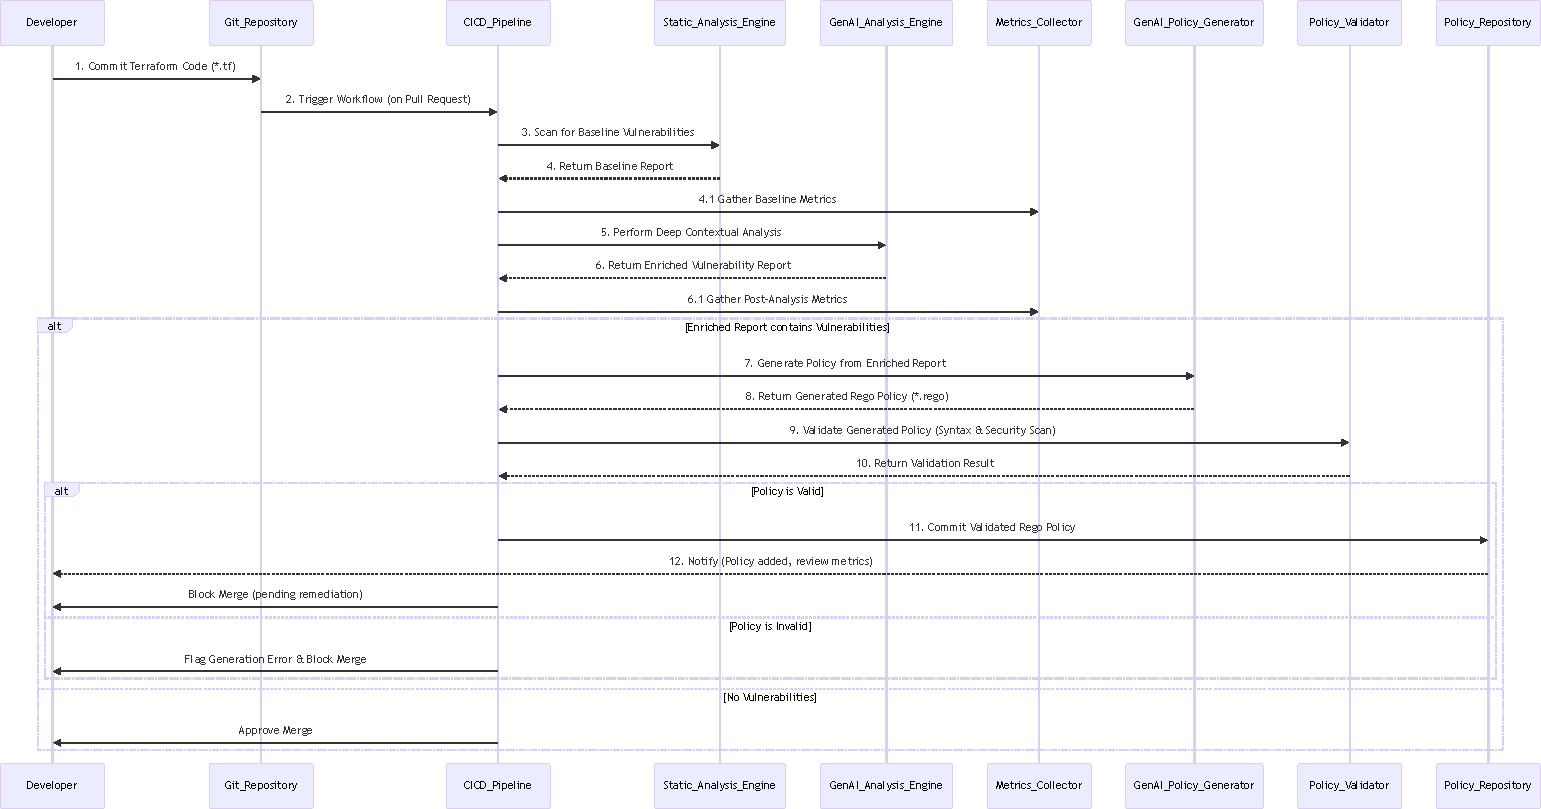
\includegraphics[width=0.9\linewidth,height=0.7\textheight,keepaspectratio]{Figures/image.pdf}
\caption{End-to-End Workflow Sequence Diagram}
\label{fig:e2e_workflow}
\end{figure}
\end{landscape}

The workflow is initiated when a user executes the main Python script from the command line, providing the path to a target Terraform (\texttt{.tf}) file as an argument. The application then proceeds through the following automated steps:

\begin{enumerate}
    \item \textbf{Static Scan:} The \textbf{\texttt{Analyzer}} module is invoked. It runs the tfsec \gls{sast} tool on the specified \gls{terraform} file to identify any known misconfigurations or vulnerabilities.
    \item \textbf{GenAI Contextual Analysis:} The structured findings from the static scan are fed into the \gls{genai} Analysis Engine (\gls{aws-bedrock}) for deep, contextual analysis to reduce \glspl{false-positive} and identify complex misconfigurations that traditional tools might miss.
    \item \textbf{Policy Generation:} The enriched vulnerability report from the \gls{genai} analysis is passed to the \gls{pg} module. This component constructs a detailed, context-rich prompt by combining the analysis findings with relevant information retrieved from the \gls{rag} \gls{kb}, then communicates with the \gls{aws-bedrock} \gls{api} to generate a targeted \gls{rego} policy specifically designed to mitigate the identified risks.
    \item \textbf{Validation:} The raw, generated \gls{rego} policy is immediately passed to the \texttt{Validator} module. This component uses the \gls{opa} toolchain to verify that the policy is syntactically correct and well-formed.
    \item \textbf{Output:} If the policy successfully passes validation, the application saves the new Rego policy as a \texttt{.rego} file to a designated output directory. The application's execution concludes by printing the path to the generated file to the console.
\end{enumerate}

This self-contained workflow from file input to policy output is designed for both interactive use by a security analyst and for integration into larger automated systems. For example, it can be executed as a script within a \gls{cicd} pipeline, where the resulting policy artifact can then be automatically committed to a repository and used as a quality gate.

\section{CI/CD \& DevSecOps Integration}

The prototype is designed to analyze Infrastructure-as-Code (IaC) configurations written in HashiCorp's Terraform. Terraform was chosen as it is a leading tool for IaC that allows for the automation of infrastructure provisioning through a strict development and review lifecycle \cite{howard_terraform_2022-1}. It supports a wide range of cloud providers, including AWS, making it a representative choice for this research.
While the prototype is a self-contained command-line tool, its primary intended application is within a \gls{cicd} pipeline to enable a proactive \gls{devsecops} workflow. This integration automates the process of security analysis and policy enforcement, "shifting left" to catch and remediate vulnerabilities before they reach production \cite{delicheh_mitigating_2024}. The implementation uses \gls{github} Actions as the \gls{cicd} platform, indicated by the presence of a \texttt{.github/workflows/main.yml} file, which enables automated testing and tracks code history. The integration is achieved through a \gls{github} Actions workflow that is triggered whenever a developer opens a pull request containing changes to \gls{terraform} files. This workflow acts as an automated quality gate and performs the following steps:
\begin{enumerate}
    \item \textbf{Code Checkout \& Setup:} The pipeline begins by checking out the source code, which is managed using \gls{git} for version control, and setting up the Python environment. This setup includes installing the dependencies from \texttt{requirements.txt} and utilizing a virtual environment (\texttt{.venv}) for isolation, guaranteeing a consistent, reproducible development and execution environment.
    \item \textbf{Execute Security Scan:} The core command-line application is executed. It is pointed at the modified Terraform files within the pull request, running the end-to-end workflow of scanning, generation, and validation.
    \item \textbf{Commit New Policy:} If the tool successfully generates a new, validated Rego policy, the workflow commits this new policy file to a dedicated directory within the repository.
    \item \textbf{Enforce Policy as a Quality Gate:} The pipeline then uses the \gls{opa} toolchain to evaluate the proposed \gls{terraform} changes against the entire set of \gls{rego} policies in the repository, including the one that was just generated. If the proposed changes violate any policy, the \gls{opa} evaluation fails.
    \item \textbf{Block or Approve:} A failure in the \gls{opa} evaluation causes the entire \gls{cicd} pipeline to fail. This automatically blocks the pull request from being merged and provides immediate feedback to the developer that their changes are not compliant with security standards. This gating mechanism ensures that only secure and compliant \gls{iac} can be merged into the main branch.
\end{enumerate}
By integrating the command-line tool in this manner, the framework moves from being a simple analysis utility to a powerful, automated control that is seamlessly embedded in the software development lifecycle.

\section{Limitations \& Trade-offs}
\label{sec:limitations_tradeoffs}

While the prototype successfully demonstrates the core concepts of \gls{genai}-driven security automation, its design and implementation involve several inherent limitations and trade-offs. These were consciously accepted to focus on the primary research questions but are important to acknowledge for a complete understanding of the system's practical applicability.
\begin{itemize}
    \item \textbf{Model Performance vs. Cost and Latency:} The choice of the \gls{llm} (Anthropic Claude on \gls{aws-bedrock}) represents a trade-off between reasoning capability, cost, and response time. While powerful, the model introduces latency into the \gls{cicd} pipeline, which could impact developer velocity in a high-frequency deployment environment. Using smaller, faster models could reduce latency and cost but might compromise the quality and accuracy of the generated policies.
    \item \textbf{Analysis Scope and State Confidentiality:} The current implementation analyzes stateless \gls{terraform} configuration files (\texttt{.tf}). It does not parse the \gls{terraform} state file (\texttt{.tfstate}), which contains the real-world state of the deployed infrastructure. This decision was made to avoid the significant security risk of handling a state file that often contains sensitive data and secrets. However, this limits the analysis, as it prevents the system from detecting configuration drift or vulnerabilities that only manifest in the deployed state.
    \item \textbf{Risk of Policy \gls{false-negative}:} While the system includes a validation step for syntactic correctness and a self-correction loop, there remains a risk of logical errors or "\gls{false-negative}" in the generated \gls{rego} policies. A policy might be syntactically valid but fail to fully or correctly mitigate the intended vulnerability. This limitation underscores the critical importance of the \gls{hitl} review process as a final safeguard against flawed automated controls.
    \item \textbf{Dependency on External Service Quotas:} The system's reliance on the \gls{aws-bedrock} service makes it subject to external factors such as service availability, regional limitations, and \gls{api} rate limits (quotas). In a large-scale enterprise environment with many parallel \gls{cicd} pipelines, high-volume usage could potentially exceed these quotas, leading to failed pipeline runs. This dependency requires careful monitoring and potentially a more resilient architecture with fallback mechanisms.
    \item \textbf{Knowledge Base Maintenance:} The effectiveness of the \gls{rag} system is directly tied to the quality and currency of its knowledge base. Keeping the documentation for \gls{terraform}, \gls{aws}, and \gls{rego} up-to-date requires a manual maintenance effort. As technologies evolve, this \gls{kb} must be actively managed to prevent the \gls{llm} from generating outdated or incorrect policies based on stale information.
\end{itemize}
% Model latency vs. cost, Terraform state confidentiality, policy false-negatives, Bedrock service quotas.

\section{Summary}

This chapter provided a comprehensive overview of the design and implementation of the prototype system for \gls{genai}-driven security automation. It detailed the translation of the conceptual framework from Chapter~\ref{chap:conceptual_framework} into a practical application, outlining the specific design objectives, technology stack, and high-level architecture. The implementation was presented as two interconnected codebases: a reproducible, secure cloud infrastructure defined in \gls{terraform}, and a modular Python application that orchestrates the end-to-end workflow. The chapter elaborated on the key architectural patterns and software engineering practices employed to ensure the system's robustness, maintainability, and quality. These include a modular architecture, a sequential pipeline for data processing, a \gls{facade-pattern} for interacting with the \gls{genai} service, and a self-correction loop for iterative refinement of the generated policies. The end-to-end workflow, from static analysis of \gls{terraform} files to the generation and validation of \gls{rego} policies, was described in detail, highlighting the seamless integration of traditional security tools with advanced \gls{ai} capabilities. Furthermore, the chapter discussed the prototype's integration into a modern \gls{devsecops} workflow, acting as an automated quality gate within a \gls{cicd} pipeline. Finally, the inherent limitations and trade-offs of the implementation were acknowledged, providing a balanced perspective on the system's practical applicability. This detailed account of the implementation serves as the foundation for the empirical evaluation presented in the following chapter.